\section{Work Mapping}

\subsection{{\tt task} and {\tt tasks} Construct}

The \|task| construct generates a task, which is executed by the specified
nodes. The \|tasks| construct asserts that surrounding \|task| constructs can be
executed in parallel.

% This page shows some examples of the task construct other than those in
% Tutorial (Global-view).

\subsubsection{{\tt task} Construct}

The \|on| clause of the \|task| construct specifies the node set that
executes the task.

\begin{XCexample}
#include <stdio.h>
#pragma xmp nodes p[4]

int main(){
  int num = xmpc_node_num();
#pragma xmp task on p[1:3]
{
  printf("%d: Hello\n", num);
}

  return 0;
}
\end{XCexample}

\begin{XFexample}
program main
!$xmp nodes p(4)
  integer :: num

  num = xmp_node_num()
!$xmp task on p(2:4)
  write(*,*) num, ": Hello"
!$xmp end task

end program main
\end{XFexample}

In the above example, nodes \|p[1]|, \|p[2]|, and \|p[3]| invokes the \|printf()|
function, and \|p[1]| outputs ``1: Hello'' in XMP/C; \|p(2)|, \|p(3)|, and \|p(4)|
execute the \|write| statement, and \|p(2)| outputs ``2: Hello'' in
XMP/Fortran.

Note that a new node set is generated by each task construct. Let's
consider inserting a \|bcast| construct into the task.

\begin{XCexample}
#pragma xmp task on p[1:3]
{
#pragma xmp bcast (num)
}
\end{XCexample}

\begin{XFexample}
!$xmp task on p(2:4)
!$xmp bcast (num)
!$xmp end task
\end{XFexample}

This \|bcast| construct is executed by the node set specified by the task
construct. Thus, the node \|p[1]| broadcasts the value to \|p[2]| and
\|p[3]| in XMP/C, and \|p(2)| to \|p(3)| and \|p(4)| in XMP/Fortran.

\begin{figure}
  \centering
  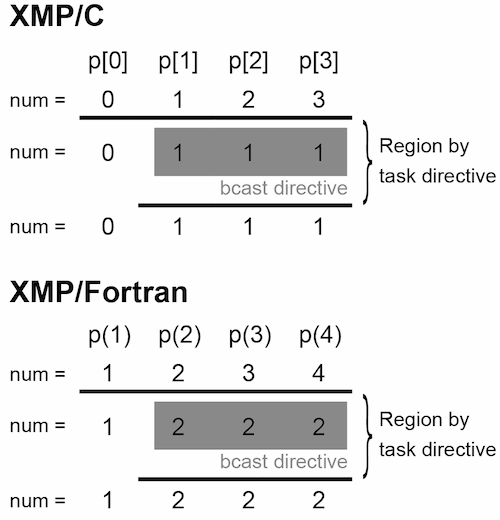
\includegraphics{figs/task.png}
\end{figure}

The \|bcast| construct in the above code is equivalent to that in the
following code, where it is executed by a new node set that is
explicitly declared.

\begin{XCexample}
#pragma xmp nodes q[3] = p[1:3]
#pragma xmp bcast (num) on q
\end{XCexample}

\begin{XFexample}
!$xmp nodes q(3) = p(2:4)
!$xmp bcast (num) on q
\end{XFexample}

Note that the task is executed by the node set specified by the \|on|
clause. Therefore, {\tt xmpc\_node\_num()} and {\tt xmp\_node\_num()}
return the id in the node set.

For example, consider inserting {\tt xmpc\_node\_num()} or {\tt
xmp\_node\_num()} into the task in the first program.

\begin{XCexample}
#include <stdio.h>
#pragma xmp nodes p[4]

int main(){
#pragma xmp task on p[1:3]
{
  printf("%d: Hello\n", xmpc_node_num());
}

  return 0;
}
\end{XCexample}

\begin{XFexample}
program main
!$xmp nodes p(4)

!$xmp task on p(2:4)
  write(*,*) xmp_node_num(), ": Hello"
!$xmp end task

end program main
\end{XFexample}

The node \|p[1]| outputs ``0: Hello'' in XMP/C, and p(2) ``1: Hello'' in XMP/Fortran.

\begin{mynote}
A new node set should be collectively generated by
all of the executing 
nodes at the point of a \|task| construct unless it is surrounded by a \|tasks|
construct. In the above example, \|p[0]| in XMP/C and \|p(1)| in XMP/Fortran
must execute the task construct.
\end{mynote}


\subsubsection{{\tt tasks} Construct}

Let's consider that each of two tasks invokes a function.

\begin{XCexample}
#pragma xmp nodes p[4]

#pragma xmp task on p[0:2]
{
  func_a();
}
#pragma xmp task on p[2:2]
{
  func_b();
}
\end{XCexample}

\begin{XFexample}
!$xmp nodes p(4)

!$xmp task on p(1:2)
  call func_a()
!$xmp end task
!$xmp task on p(3:4)
  call func_b()
!$xmp end task
\end{XFexample}

In the above example, the two tasks cannot be executed in parallel
because those \|on| clauses must be evaluated by all of the executing
nodes.

\begin{figure}
  \centering
  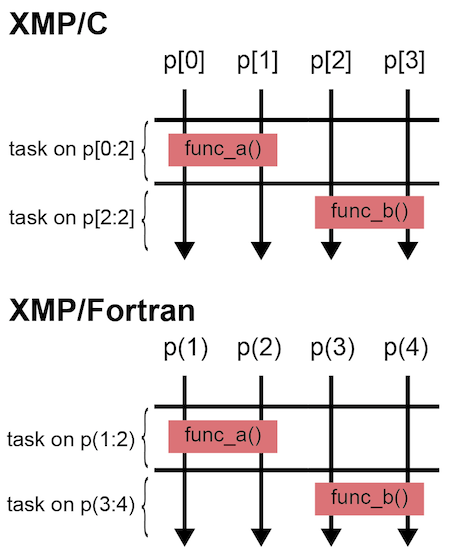
\includegraphics{figs/task_noparallel.png}
\end{figure}

Use the \|tasks| construct to execute multiple tasks in parallel.

\begin{XCexample}
#pragma xmp nodes p[4]

#pragma xmp tasks
{
#pragma xmp task on p[0:2]
{
  func_a();
}
#pragma xmp task on p[2:2]
{
  func_b();
}
}
\end{XCexample}

\begin{XFexample}
!$xmp nodes p(4)

!$xmp tasks
!$xmp task on p(1:2)
  call func_a()
!$xmp end task
!$xmp task on p(3:4)
  call func_b()
!$xmp end task
!$xmp end tasks
\end{XFexample}

Because the node sets specified by the \|on| clauses of the \|task|
constructs surrounded by a \|tasks| construct are disjoint, they can be
executed in parallel.

\begin{figure}
  \centering
  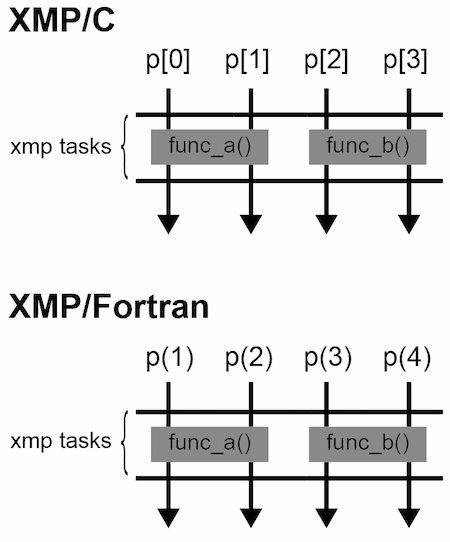
\includegraphics{figs/tasks.png}
\end{figure}


\subsection{{\tt loop} Construct}

The \|loop| construct is used to parallelize a loop. Distributed arrays in
such a loop must fulfill the following two conditions:

\begin{enumerate}
  \item There is no data/control dependence among the iterations. In other
words, the iterations of the loop can be executed in any order to
produce the same result.
  \item An element of a distributed array is accessed only by the node that owns
the element.
\end{enumerate}

\subsubsection{Accessing Distributed Array}

The programs below are examples of a right \|loop| directive and a loop
statement. The condition 1. is satisfied because \|i| is the only one index
of the distributed array \|a| that is accessed within the loop, and the
condition 2 is also satisfied because the indices of the template in the
\|on| clause of the loop directive is identical to that of the distributed
array.

\begin{XCexample}
#pragma xmp nodes p[2]
#pragma xmp template t[10]
#pragma xmp distribute t[block] onto p

int main(){
  int a[10];
#pragma xmp align a[i] with t[i]

#pragma xmp loop on t[i]
  for(int i=0;i<10;i++)
    a[i] = i;

  return 0;
}
\end{XCexample}

\begin{XFexample}
program main
!$xmp nodes p(2)
!$xmp template t(10)
!$xmp distribute t(block) onto p
  integer a(10)
!$xmp align a(i) with t(i)

!$xmp loop on t(i)
  do i=1, 10
    a(i) = i
  enddo

end program main
\end{XFexample}

\begin{figure}
  \centering
  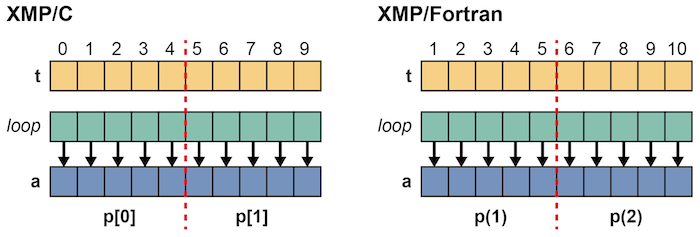
\includegraphics[width=\textwidth]{figs/loop1.png}
\end{figure}

Is it possible to parallelize the below loops whose bounds are shrunk?

\begin{XCexample}
#pragma xmp loop on t[i]
  for(int i=1;i<9;i++)
    a[i] = i;
\end{XCexample}

\begin{XFexample}
!$xmp loop on t(i)
  do i=2, 9
    a(i) = i
  enddo
\end{XFexample}

In this case, the conditions 1 and 2 are satisfied and therefore it is
possible to parallelize them. In XMP/C, \|p[0]| processes the indices from
one to four and \|p[1]| from five to eight. In XMP/Fortran, \|p(1)| processes
the indices from two to five and \|p(2)| from six to nine.

\begin{figure}
  \centering
  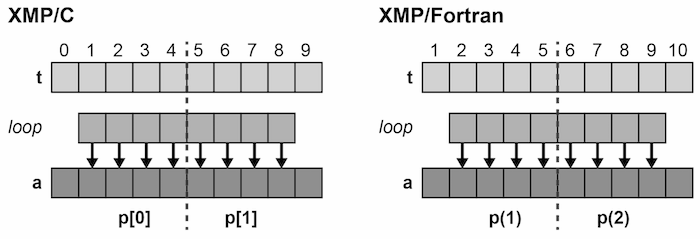
\includegraphics[width=\textwidth]{figs/loop2.png}
\end{figure}

Next, is it possible to parallelize the below loops in which the index
of the distributed array is different?

\begin{XCexample}
#pragma xmp loop on t[i]
  for(int i=1;i<9;i++)
    a[i+1] = i;
\end{XCexample}

\begin{XFexample}
!$xmp loop on t(i)
  do i=2, 9
    a(i+1) = i
  enddo
\end{XFexample}

In this case, the condition 1 is satisfied but 2 is not, and therefore
it is not possible to parallelize them. In XMP/C, \|p[0]| tries to access
\|a[5]| but does not own it. In XMP/Fortran, \|p(1)| tries to access
\|a(6)| but does not own it.

\begin{figure}
  \centering
  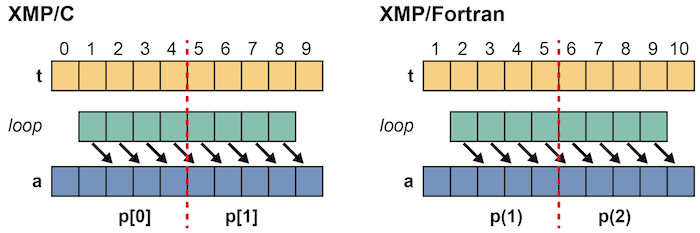
\includegraphics[width=\textwidth]{figs/loop3.png}
\end{figure}


\subsubsection{Reduction Computation}

The serial programs below are examples of the reduction computation.

\begin{Cexample}
#include <stdio.h>

int main(){
  int a[10], sum = 0;

  for(int i=0;i<10;i++){
    a[i] = i+1;
    sum += a[i];
  }

  printf("%d\n", sum);

  return 0;
}
\end{Cexample}

\begin{Fexample}
program main
  integer :: a(10), sum = 0

  do i=1, 10
    a(i) = i
    sum = sum + a(i)
  enddo

  write(*,*) sum

end program main
\end{Fexample}

If the above loops are parallelized only with the \|loop| directive, the
value of the variable \|sum| varies from node to node because it is
calculated separately on each node.

\begin{XCexample}
#pragma xmp loop on t[i]
   for(int i=0;i<10;i++){
     a[i] = i+1;
     sum += a[i];
   }
\end{XCexample}

\begin{XFexample}
!$xmp loop on t(i)
  do i=1, 10
    a(i) = i
    sum = sum + a(i)
  enddo
\end{XFexample}

\begin{figure}
  \centering
  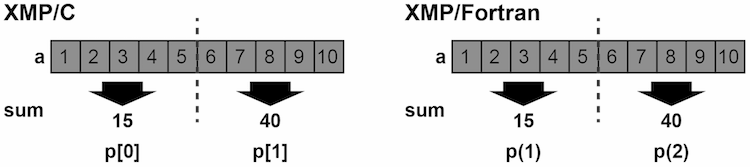
\includegraphics[width=\textwidth]{figs/reduction1.png}
\end{figure}

Then, add the \|reduction| clause to the \|loop| directive.

\begin{XCexample}
#include <stdio.h>
#pragma xmp nodes p[2]
#pragma xmp template t[10]
#pragma xmp distribute t[block] onto p

int main(){
  int a[10], sum = 0;
#pragma xmp align a[i] with t[i]

#pragma xmp loop on t[i] reduction(+:sum)
  for(int i=0;i<10;i++){
    a[i] = i+1;
    sum += a[i];
  }

  printf("%d\n", sum);

  return 0;
}
\end{XCexample}

\begin{XFexample}
program main
!$xmp nodes p(2)
!$xmp template t(10)
!$xmp distribute t(block) onto p
  integer :: a(10), sum = 0
!$xmp align a(i) with t(i)

!$xmp loop on t(i) reduction(+:sum)
  do i=1, 10
    a(i) = i
    sum = sum + a(i)
  enddo

  write(*,*) sum

end program main
\end{XFexample}

An operator and target variables for reduction are specified in a
\|reduction| clause. In the above examples, a ``\|+|'' operator is
specified for the reduction computation to produce a total sum among nodes.

\begin{figure}
  \centering
  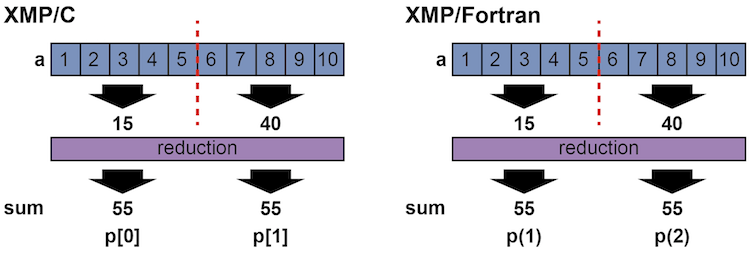
\includegraphics[width=\textwidth]{figs/reduction2.png}
\end{figure}

Operations that can be used in a reduction computation are limited to
the following associative ones.

\begin{Cexample}
+
*
-
&
|
^
&&
||
max
min
firstmax
firstmin
lastmax
lastmin
\end{Cexample}

\begin{Fexample}
+
*
-
.and.
.or.
.eqv.
.neqv.
max
min
iand
ior
ieor
firstmax
firstmin
lastmax
lastmin
\end{Fexample}

\begin{mynote}
  If the reduction variable is a type of floating
  point, the difference of the order of the executions can make a little
  bit difference between serial and parallel executions.
\end{mynote}


\subsubsection{Parallelizing Nested Loop}

Parallelization of nested loops can be specified similarly for a single
one.

\begin{XCexample}
#pragma xmp nodes p[2][2]
#pragma xmp template t[10][10]
#pragma xmp distribute t[block][block] onto p

int main(){
  int a[10][10];
#pragma xmp align a[i][j] with t[i][j]

#pragma xmp loop on t[i][j]
  for(int i=0;i<10;i++)
    for(int j=0;j<10;j++)
      a[i][j] = i*10+j;

  return 0;
}
\end{XCexample}

\begin{XFexample}
program main
!$xmp nodes p(2,2)
!$xmp template t(10,10)
!$xmp distribute t(block,block) onto p
  integer :: a(10,10)
!$xmp align a(j,i) with t(j,i)

!$xmp loop on t(j,i)
  do i=1, 10
    do j=1, 10
      a(j,i) = i*10+j
    enddo
  enddo

end program main
\end{XFexample}


\subsection{{\tt array} Construct}

The \|array| construct is for work mapping of array assignment statements.

\begin{XCexample}
#pragma xmp align a[i] with t[i]
  :
#pragma xmp array on t[0:N]
a[0:N] = 1.0;
\end{XCexample}

\begin{XFexample}
!$xmp align a(i) with t(i)
  :
!$xmp array on t(1:N)
a(1:N) = 1.0
\end{XFexample}

The above is equivalent to the below.

\begin{XCexample}
#pragma xmp align a[i] with t[i]
  :
#pragma xmp loop on t[i]
for(int i=0;i<N;i++)
  a[i] = 1.0;
\end{XCexample}

\begin{XFexample}
!$xmp align a(i) with t(i)
  :
!$xmp loop on t(i)
do i=1, N
  a(i) = 1.0
enddo
\end{XFexample}

This construct can also be applied to multi-dimensional arrays. The
triplet notation enables specifying operations for all elements of the
array.

\begin{XCexample}
#pragma xmp align a[i][j] with t[i][j]
  :
#pragma xmp array on t[:][:]
a[:][:] = 1.0;
\end{XCexample}

\begin{XFexample}
!$xmp align a(j,i) with t(j,i)
  :
!$xmp array on t(:,:)
a(:,:) = 1.0
\end{XFexample}

\begin{mynote}
The template appearing in the \|on| clause must have
the same shape of
arrays in the following statement. The right-hand side value must be
identical among all nodes because the array construct is a global
  (i.e. collective) operation.
\end{mynote}
